\section*{7.3 Distribuições a Priori Conjugadas}
Para cada um dos modelos estatísticos mais populares, existe uma família de distribuições para o parâmetro com uma propriedade muito especial. Se a distribuição a priori for escolhida como um membro dessa família, então a distribuição a posteriori também será um membro da mesma família. Tal família de distribuições é chamada de \textit{família conjugada}. A escolha de uma distribuição a priori de uma família conjugada tornará o cálculo da distribuição a posteriori particularmente simples.

\subsection*{Amostragem de uma Distribuição de Bernoulli}

\noindent\textbf{Exemplo 7.3.1} \quad \textbf{Um Ensaio Clínico.} No Exemplo 5.8.5 (página 330), estávamos observando pacientes em um ensaio clínico. A proporção $P$ de resultados bem-sucedidos entre todos os pacientes possíveis era uma variável aleatória para a qual escolhemos uma distribuição da família de distribuições beta. Essa escolha tornou o cálculo da distribuição condicional de $P$ dados os dados observados muito simples no final daquele exemplo. De fato, a distribuição condicional de $P$ dados os dados era outro membro da família beta.

O resultado do Exemplo 7.3.1 ocorre em geral e é o assunto do próximo teorema.

\vspace{1cm}
\noindent\textbf{Teorema 7.3.1} \quad Suponha que $X_1, \dots, X_n$ formem uma amostra aleatória da distribuição de Bernoulli com parâmetro $\theta$, que é desconhecido $(0 < \theta < 1)$. Suponha também que a distribuição a priori de $\theta$ seja a distribuição beta com parâmetros $\alpha > 0$ e $\beta > 0$. Então a distribuição a posteriori de $\theta$ dado $X_i = x_i \, (i=1, \dots, n)$ é a distribuição beta com parâmetros $\alpha + \sum_{i=1}^{n}x_i$ e $\beta + n - \sum_{i=1}^{n}x_i$.

O Teorema 7.3.1 é apenas uma reafirmação do Teorema 5.8.2 (página 329), e sua prova é essencialmente o cálculo no Exemplo 5.8.3.

\subsubsection*{Atualizando a Distribuição a Posteriori}
Uma implicação do Teorema 7.3.1 é a seguinte: Suponha que a proporção $\theta$ de itens defeituosos em um grande lote seja desconhecida, a distribuição a priori de $\theta$ seja a distribuição beta com parâmetros $\alpha$ e $\beta$, e os itens sejam selecionados um de cada vez aleatoriamente do lote. Suponha que o primeiro item inspecionado seja defeituoso, a distribuição a posteriori de $\theta$ será a distribuição beta com parâmetros $\alpha+1$ e $\beta$. Se o primeiro item não for defeituoso, a distribuição a posteriori será a distribuição beta com parâmetros $\alpha$ e $\beta+1$. O processo pode ser continuado da seguinte maneira: a cada item inspecionado, a distribuição a posteriori atual de $\theta$ é trocada por uma nova distribuição beta na qual o valor de ou o parâmetro $\alpha$ ou o parâmetro $\beta$ é aumentado em uma unidade, a cada vez que um item defeituoso é encontrado, e o valor do parâmetro $\beta$ é aumentado em uma unidade a cada vez que um item não defeituoso é encontrado.

\vspace{1cm}
\noindent\textbf{Definição 7.3.1} \quad \textbf{Família Conjugada/Hiperparâmetros.} Seja $\mathcal{F}$ uma família de possíveis distribuições sobre um espaço de parâmetros $\Omega$. Suponha que, não importa qual observação $\mathbf{X}=(X_1, \dots, X_n)$ observarmos, nem qual distribuição a priori $\xi \in \mathcal{F}$ escolhermos, a distribuição a posteriori $\xi(\theta|\mathbf{x})$ é um membro de $\mathcal{F}$. Então $\mathcal{F}$ é chamada de \textit{família conjugada} de distribuições para amostras das distribuições $f(x|\theta)$. Suponha também que a família $\mathcal{F}$ seja parametrizada por outros parâmetros, então os parâmetros associados para a distribuição a priori são chamados de \textit{hiperparâmetros}, e os parâmetros associados da distribuição a posteriori são chamados de \textit{hiperparâmetros a posteriori}.

\vspace{1cm}
O Teorema 7.3.1 diz que a família de distribuições beta é uma família conjugada de distribuições a priori para amostras de uma distribuição de Bernoulli. Se uma distribuição a priori é uma distribuição beta, então a distribuição a posteriori em cada estágio de amostragem também será uma distribuição beta, independentemente dos valores da amostra observados. Os parâmetros $\alpha$ e $\beta$ na distribuição a priori do Teorema 7.3.1 são os hiperparâmetros. Os correspondentes hiperparâmetros a posteriori de $\theta$ são $\alpha + \sum_{i=1}^{n}x_i$ e $\beta+n-\sum_{i=1}^{n}x_i$. A estatística $\sum_{i=1}^{n}X_i$ é necessária para calcular a distribuição a posteriori, portanto, ela estará presente em qualquer inferência baseada na distribuição a posteriori. Exercícios 23 e 24 introduzem uma coleção geral de f.p.s e f.d.p.s $f(x|\theta)$ para as quais as famílias de distribuições conjugadas existem. A maioria das famílias de distribuições nomeadas abordadas por esses exercícios são notáveis exceções.

\vspace{1cm}
\noindent\textbf{Exemplo 7.3.2} \quad \textbf{A Variância da Distribuição Beta a Posteriori.} Suponha que a proporção $\theta$ de itens defeituosos em um grande lote seja desconhecida, a distribuição a priori de $\theta$ seja a distribuição uniforme no intervalo $[0, 1]$, e os itens devam ser selecionados aleatoriamente do lote e inspecionados até que a variância da distribuição a posteriori de $\theta$ tenha sido reduzida a 0.01 ou menos. Devemos determinar o número total de itens defeituosos e não defeituosos que devem ser obtidos antes que o processo de amostragem seja interrompido.
Conforme afirmado na Seção 5.8, a distribuição uniforme no intervalo $[0, 1]$ é a distribuição beta com parâmetros 1 e 1. Portanto, depois que $y$ itens defeituosos e $z$ itens não defeituosos tiverem sido obtidos, a distribuição a posteriori de $\theta$ será a distribuição beta com $\alpha=y+1$ e $\beta=z+1$. Foi mostrado no Teorema 5.8.3 que a variância da distribuição beta com parâmetros $\alpha$ e $\beta$ é $\alpha\beta/ [(\alpha+\beta)^2(\alpha+\beta+1)]$. Portanto, a variância $V$ da distribuição a posteriori de $\theta$ será
$$ V = \frac{(y+1)(z+1)}{(y+z+2)^2(y+z+3)}. $$
A amostragem deve parar assim que o número de defeituosos $y$ e o número de não defeituosos $z$ que foram obtidos sejam tais que $V \le 0.01$. Pode ser mostrado (ver Exercício 2) que não será necessário selecionar mais de 22 itens, mas é necessário selecionar pelo menos sete itens.

\vspace{1cm}
\noindent\textbf{Exemplo 7.3.3} \quad \textbf{Uso de Luvas por Enfermeiras.} Friedland et al. (1992) estudaram 23 enfermeiras em um hospital do centro da cidade antes e depois de um programa educacional sobre a importância de usar luvas. Eles registraram se as enfermeiras usavam ou não luvas em procedimentos nos quais poderiam entrar em contato com fluidos corporais. Antes do programa educacional, as enfermeiras foram observadas durante 51 procedimentos, e usaram luvas em apenas 13 deles. Seja $\theta$ a probabilidade de uma enfermeira usar luvas dois meses após o programa educacional. Podemos estar interessados em como $\theta$ se compara a 13/51, a proporção observada antes do programa.
Vamos considerar duas distribuições a priori diferentes para $\theta$ para ver quão sensível a distribuição a posteriori de $\theta$ é à escolha da distribuição a priori. A primeira distribuição a priori será uniforme no intervalo $[0, 1]$, que também é a distribuição beta com parâmetros 1 e 1. A segunda distribuição a priori será a distribuição beta com parâmetros 13 e 38. Esta segunda distribuição a priori tem uma variância muito menor que a primeira e tem sua média em 13/51. Alguém que sustenta a segunda priori acredita firmemente que o programa educacional não terá efeito perceptível.
Dois meses após o programa educacional, 56 procedimentos foram observados, com as enfermeiras usando luvas em 50 deles. A distribuição a posteriori de $\theta$, com base na primeira priori, seria a distribuição beta com parâmetros $1+50=51$ e $1+6=7$. Em particular, a média a posteriori de $\theta$ é $51/(51+7)=0.88$, e a probabilidade a posteriori de que $\theta > 13/51$ é essencialmente 1. Com base na segunda priori, a distribuição a posteriori de $\theta$ seria a distribuição beta com parâmetros $13+50=63$ e $38+6=44$. A média a posteriori seria $63/(63+44)=0.59$, e a probabilidade a posteriori de que $\theta > 13/51$ é $0.95$. Assim, mesmo alguém que era inicialmente cético sobre o programa educacional parece ter sido convencido. A probabilidade é bastante alta de que as enfermeiras tenham pelo menos o dobro de probabilidade de usar luvas após o programa como antes.
A Figura 7.3 mostra as f.d.p.s de ambas as distribuições a posteriori calculadas acima. As distribuições são claramente muito diferentes. Por exemplo, a primeira dá uma probabilidade maior que 0.99 de que $\theta>0.7$, enquanto a segunda dá uma probabilidade menor que $0.001$ de que $\theta>0.7$. No entanto, uma vez que estamos apenas interessados na probabilidade de que $\theta > 13/51=0.5098$, vemos que ambas as prioris concordam que essa probabilidade é bastante grande.

\vspace{1cm}
\begin{figure}[H]

\centering

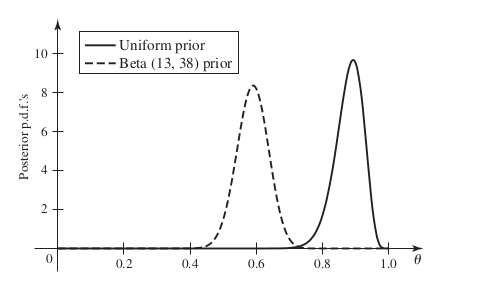
\includegraphics[width=0.5\textwidth]{img/7_3/img_1.png}

\end{figure}\vspace{1cm}

\subsection*{Amostragem de uma Distribuição de Poisson}

\noindent\textbf{Exemplo 7.3.4} \quad \textbf{Chegadas de Clientes.} O dono de uma loja modela as chegadas de clientes como um processo de Poisson com uma taxa desconhecida de $\theta$ por hora. Ele atribui a $\theta$ uma distribuição gama com parâmetros 3 e 2. Seja $X$ o número de clientes que chegam em um período específico de uma hora. Se $X=3$ for observado, o dono da loja quer atualizar a distribuição de $\theta$.

\vspace{1cm}
Quando as amostras são retiradas de uma distribuição de Poisson, a família de distribuições gama é uma família conjugada de distribuições a priori. Essa relação é mostrada no próximo teorema.

\vspace{1cm}
\noindent\textbf{Teorema 7.3.2} \quad Suponha que $X_1, \dots, X_n$ formem uma amostra aleatória da distribuição de Poisson com média $\theta > 0$, e $\theta$ seja desconhecido. Suponha também que a distribuição a priori de $\theta$ seja a distribuição gama com parâmetros $\alpha > 0$ e $\beta > 0$. Então a distribuição a posteriori de $\theta$, dado que $X_i=x_i \, (i=1, \dots, n)$, é a distribuição gama com parâmetros $\alpha + \sum_{i=1}^{n}x_i$ e $\beta + n$.

\vspace{1cm}
\noindent\textbf{Prova} \quad Seja $y=\sum_{i=1}^{n}x_i$. Então a função de verossimilhança $f_n(\mathbf{x}|\theta)$ satisfaz a relação
$$ f_n(\mathbf{x}|\theta) \propto e^{-n\theta}\theta^y. $$
Nesta relação, um fator que envolve $\mathbf{x}$ mas não depende de $\theta$ foi descartado do lado direito. Além disso, a f.d.p. a priori de $\theta$ tem a forma
$$ \xi(\theta) \propto \theta^{\alpha-1}e^{-\beta\theta} \quad \text{para } \theta>0. $$
Como a f.d.p. a posteriori $\xi(\theta|\mathbf{x})$ é proporcional a $f_n(\mathbf{x}|\theta)\xi(\theta)$, segue-se que
$$ \xi(\theta|\mathbf{x}) \propto \theta^{\alpha+y-1}e^{-(\beta+n)\theta} \quad \text{para } \theta>0. $$
O lado direito desta relação pode ser reconhecido como sendo, exceto por um fator constante, a f.d.p. da distribuição gama com parâmetros $\alpha+y$ e $\beta+n$. Portanto, a distribuição a posteriori de $\theta$ é como especificado no teorema. \rule{0.5em}{0.5em}

\vspace{1cm}
No Teorema 7.3.2, os números $\alpha$ e $\beta$ são os hiperparâmetros a priori. Note que os hiperparâmetros a posteriori são $\alpha + \sum_{i=1}^{n}x_i$ e $\beta+n$. Note que a estatística $Y=\sum_{i=1}^{n}X_i$ é usada para calcular a distribuição a posteriori de $\theta$, e, portanto, fará parte de qualquer inferência baseada na posteriori.

\vspace{1cm}
\noindent\textbf{Exemplo 7.3.5} \quad \textbf{Chegadas de Clientes.} No Exemplo 7.3.4, podemos aplicar o Teorema 7.3.2 com $n=1, \alpha=3, \beta=2$, e $x_1=3$. A distribuição a posteriori de $\theta$ dado $X=3$ é a distribuição gama com parâmetros 6 e 3.

\vspace{1cm}
\noindent\textbf{Exemplo 7.3.6} \quad \textbf{A Variância da Distribuição Gama a Posteriori.} Considere uma distribuição de Poisson para a qual a média $\theta$ é desconhecida, e suponha que a f.d.p. a priori de $\theta$ seja a seguinte:
$$ \xi(\theta) = 
\begin{cases}
2e^{-2\theta} & \text{para } \theta>0, \\
0 & \text{para } \theta \le 0.
\end{cases}
$$
Suponha também que as observações devam ser retiradas da distribuição de Poisson até que a variância da distribuição a posteriori de $\theta$ tenha sido reduzida a 0.01 ou menos. Devemos determinar o número de observações que devem ser feitas antes que o processo de amostragem seja interrompido.
A f.d.p. a priori dada é a da distribuição gama com hiperparâmetros $\alpha=1$ e $\beta=2$. Portanto, depois de termos obtido valores observados $x_1, \dots, x_n$, a soma dos quais é $y=\sum_{i=1}^{n}x_i$, a distribuição a posteriori de $\theta$ será a distribuição gama com hiperparâmetros $y+1$ e $n+2$. Foi mostrado no Teorema 5.4.2 que a variância da distribuição gama com parâmetros $\alpha$ e $\beta$ é $\alpha/\beta^2$. Portanto, a variância $V$ da distribuição a posteriori de $\theta$ será
$$ V = \frac{y+1}{(n+2)^2}. $$
A amostragem deve parar assim que os valores observados $x_1, \dots, x_n$ forem tais que $V \le 0.01$. Ao contrário do Exemplo 7.3.2, não há limite uniforme sobre quão grande $n$ precisa ser porque $y$ pode ser arbitrariamente grande, não importa qual seja $n$. Claramente, são necessárias pelo menos $n=8$ observações antes que $V \le 0.01$.

\subsection*{Amostragem de uma Distribuição Normal}

\noindent\textbf{Exemplo 7.3.7} \quad \textbf{Emissões Automotivas.} Considere novamente o exemplo de emissões automotivas em Exemplo 5.6.1 na página 302. Antes de observar os dados, suponha que um engenheiro acreditasse que cada medida de emissão tinha a distribuição normal com média $\theta$ e desvio padrão 0.5, mas que $\theta$ era desconhecido. O engenheiro também acredita que $\theta$ tem uma distribuição normal com média 2.0 e desvio padrão 1.0. Depois de ver os dados na Fig. 5.1, como este engenheiro descreveria sua incerteza sobre $\theta$?

\vspace{1cm}
Quando as amostras são retiradas de uma distribuição normal para a qual o valor da média $\theta$ é desconhecido mas o valor da variância $\sigma^2$ é conhecido, a família de distribuições normais é uma família conjugada de distribuições a priori, como mostrado no próximo teorema.

\vspace{1cm}
\noindent\textbf{Teorema 7.3.3} \quad Suponha que $X_1, \dots, X_n$ formem uma amostra aleatória de uma distribuição normal para a qual o valor da média $\theta$ é desconhecido e o valor da variância $\sigma^2 > 0$ é conhecido. Suponha também que a distribuição a priori de $\theta$ seja uma distribuição normal com média $\mu_0$ e variância $\nu_0^2$. Então a distribuição a posteriori de $\theta$ dado que $X_i=x_i \, (i=1, \dots, n)$ é a distribuição normal com média $\mu_1$ e variância $\nu_1^2$, onde
\begin{equation}
\mu_1 = \frac{\sigma^2\mu_0+n\nu_0^2\bar{x}_n}{\sigma^2+n\nu_0^2} \tag{7.3.1}
\end{equation}
e
\begin{equation}
\nu_1^2 = \frac{\sigma^2\nu_0^2}{\sigma^2+n\nu_0^2}. \tag{7.3.2}
\end{equation}

\noindent\textbf{Prova} \quad A função de verossimilhança, $f_n(\mathbf{x}|\theta)$ tem a forma
$$ f_n(\mathbf{x}|\theta) \propto \exp\left[-\frac{1}{2\sigma^2}\sum_{i=1}^{n}(x_i-\theta)^2\right]. $$
Aqui, um fator constante foi descartado do lado direito. O método de completar o quadrado (ver Exercício 24 na Seção 5.6) nos diz que
$$ \sum_{i=1}^{n}(x_i-\theta)^2 = n(\theta-\bar{x}_n)^2 + \sum_{i=1}^{n}(x_i-\bar{x}_n)^2. $$
Omitindo um fator que envolve $x_1, \dots, x_n$ mas não depende de $\theta$, podemos reescrever $f_n(\mathbf{x}|\theta)$ na seguinte forma:
$$ f_n(\mathbf{x}|\theta) \propto \exp\left[-\frac{n}{2\sigma^2}(\theta-\bar{x}_n)^2\right]. $$
Como a f.d.p. a priori $\xi(\theta)$ tem a forma
$$ \xi(\theta) \propto \exp\left[-\frac{1}{2\nu_0^2}(\theta-\mu_0)^2\right], $$
segue-se que a f.d.p. a posteriori $\xi(\theta|\mathbf{x})$ satisfaz a relação
$$ \xi(\theta|\mathbf{x}) \propto \exp\left\{-\frac{1}{2}\left[\frac{n}{\sigma^2}(\theta-\bar{x}_n)^2+\frac{1}{\nu_0^2}(\theta-\mu_0)^2\right]\right\}. $$
Se $\mu_1$ e $\nu_1^2$ são como especificado nas Eqs. (7.3.1) e (7.3.2), completar o quadrado novamente estabelece a seguinte identidade:
$$ \frac{n}{\sigma^2}(\theta-\bar{x}_n)^2+\frac{1}{\nu_0^2}(\theta-\mu_0)^2 = \frac{1}{\nu_1^2}(\theta-\mu_1)^2 + \frac{n}{\sigma^2+n\nu_0^2}(\bar{x}_n-\mu_0)^2. $$
Como o termo final no lado direito desta equação não envolve $\theta$, ele pode ser absorvido na constante de proporcionalidade, e obtemos a relação
$$ \xi(\theta|\mathbf{x}) \propto \exp\left[-\frac{1}{2\nu_1^2}(\theta-\mu_1)^2\right]. $$
O lado direito desta relação pode ser reconhecido como sendo, exceto por um fator constante, a f.d.p. da distribuição normal com média $\mu_1$ e variância $\nu_1^2$. Portanto, a distribuição a posteriori de $\theta$ é como especificado no teorema. \rule{0.5em}{0.5em}

\vspace{1cm}
No Teorema 7.3.3, os números $\mu_0$ e $\nu_0^2$ são os hiperparâmetros a priori, enquanto $\mu_1$ e $\nu_1^2$ são os hiperparâmetros a posteriori. Note que a estatística $\bar{X}_n$ é usada na construção da distribuição a posteriori, e, portanto, desempenhará um papel em qualquer inferência baseada na posteriori.

\vspace{1cm}
\noindent\textbf{Exemplo 7.3.8} \quad \textbf{Emissões Automotivas.} Podemos aplicar o Teorema 7.3.3 para responder à pergunta no final do Exemplo 7.3.7. Na notação do teorema, temos $n=46, \sigma^2=0.5^2=0.25, \mu_0=2$ e $\nu_0^2=1.0$. A média das 46 medições é $\bar{x}_n=1.329$. A distribuição a posteriori de $\theta$ é então a distribuição normal com média e variância dadas por
$$ \mu_1 = \frac{0.25 \times 2 + 46 \times 1 \times 1.329}{0.25+46\times 1} = 1.333, $$
$$ \nu_1^2 = \frac{0.25 \times 1}{0.25+46\times 1} = 0.0054. $$
A média $\mu_1$ da distribuição a posteriori de $\theta$, como dada na Eq. (7.3.1), pode ser reescrita da seguinte forma:
\begin{equation}
\mu_1 = \frac{\sigma^2}{\sigma^2+n\nu_0^2}\mu_0 + \frac{n\nu_0^2}{\sigma^2+n\nu_0^2}\bar{x}_n. \tag{7.3.3}
\end{equation}
Pode-se ver da Eq. (7.3.3) que $\mu_1$ é uma média ponderada da média a priori $\mu_0$ e da média amostral $\bar{x}_n$. Além disso, pode-se ver que o peso relativo dado a $\bar{x}_n$ satisfaz as três propriedades a seguir: (1) Para valores fixos de $\nu_0^2$ e $\sigma^2$, quanto maior o tamanho da amostra $n$, maior será o peso relativo dado a $\bar{x}_n$. (2) Para valores fixos de $\nu_0^2$ e $n$, quanto maior a variância $\sigma^2$ de cada observação na amostra, menor será o peso relativo dado a $\bar{x}_n$. (3) Para valores fixos de $\sigma^2$ e $n$, quanto maior a variância $\nu_0^2$ da distribuição a priori, maior será o peso relativo dado a $\bar{x}_n$.
Além disso, pode-se ver da Eq. (7.3.2) que a variância $\nu_1^2$ da distribuição a posteriori de $\theta$ depende do número $n$ de observações que foram feitas, mas não depende das magnitudes dos valores observados. Portanto, para uma amostra aleatória de $n$ observações a ser retirada de uma distribuição normal para a qual o valor da média $\theta$ é desconhecido, o valor da variância é conhecido, e a distribuição a priori de $\theta$ é uma distribuição normal especificada. Então, antes de qualquer observação ter sido feita, podemos usar a Eq. (7.3.2) para calcular o valor da variância $\nu_1^2$ da distribuição a posteriori. No entanto, o valor da média $\mu_1$ da distribuição a posteriori dependerá dos valores observados que são obtidos na amostra. O fato de a variância a posteriori não depender dos valores observados deve-se à suposição de que a variância $\sigma^2$ das observações individuais é conhecida. Na Seção 8.6, relaxaremos essa suposição.

\vspace{1cm}
\noindent\textbf{Exemplo 7.3.9} \quad \textbf{A Variância da Distribuição Normal a Posteriori.} Suponha que as observações devam ser retiradas de uma distribuição normal com média $\theta$ e variância 1, e que o valor de $\theta$ seja desconhecido. Suponha também que a distribuição a priori de $\theta$ seja uma distribuição normal com variância 4. Além disso, as observações devem ser feitas até que a variância da distribuição a posteriori de $\theta$ tenha sido reduzida a 0.01 ou menos. Devemos determinar o número de observações que devem ser feitas antes que o processo de amostragem seja interrompido.
Segue-se da Eq. (7.3.2) que, após $n$ observações terem sido feitas, a variância $\nu_1^2$ da distribuição a posteriori será
$$ \nu_1^2 = \frac{4}{4n+1}. $$
Portanto, a relação $\nu_1^2 \le 0.01$ será satisfeita se e somente se $n \ge 99.75$. Portanto, a variância a posteriori será de 0.01 ou menos depois de 100 observações terem sido feitas e não antes.

\vspace{1cm}
\noindent\textbf{Exemplo 7.3.10} \quad \textbf{Contagem de Calorias em Alimentos Preparados.} Allison, Heshka, Sepulveda e Heymsfield (1993) amostraram 20 alimentos preparados nacionalmente e compararam o conteúdo de calorias declarado com o conteúdo de calorias determinado no laboratório. A Figura 7.4 é um histograma das diferenças percentuais entre as medições observadas em laboratório e o conteúdo de calorias anunciado nos rótulos dos alimentos. Suponha que modelamos a distribuição condicional das diferenças dado $\theta$ como a distribuição normal com média $\theta$ e variância 100. (Nesta seção, assumimos que a variância é conhecida. Na Seção 8.6, seremos capazes de lidar com o caso em que tanto a média quanto a variância são tratadas como variáveis aleatórias com uma distribuição conjunta.) Usaremos uma distribuição a priori para $\theta$ que é a distribuição normal com média 0 e uma variância de 60. Os dados $\mathbf{X}$ compreendem as 20 diferenças na Fig. 7.4, cuja média é 0.125. A distribuição a posteriori de $\theta$ seria então a distribuição normal com média
$$ \mu_1 = \frac{100 \times 0 + 20 \times 60 \times 0.125}{100+20\times 60} = 0.1154, $$
e variância
$$ \nu_1^2 = \frac{100 \times 60}{100+20\times 60} = 4.62. $$
Por exemplo, podemos estar interessados em saber se os empacotadores estão subestimando sistematicamente as calorias em seus alimentos em pelo menos 1 por cento. Isso corresponderia a $\theta > 1$. Usando o Teorema 5.6.6, podemos encontrar
$$ \Pr(\theta > 1|\mathbf{x}) = 1 - \Phi\left(\frac{1-0.1154}{\sqrt{4.62}}\right) = 1-\Phi(1.12) = 0.3403. $$
Há uma chance não desprezível, mas não esmagadora, de que os empacotadores estejam omitindo um por cento ou mais de suas calorias dos rótulos.

\vspace{1cm}
\begin{figure}[H]

\centering

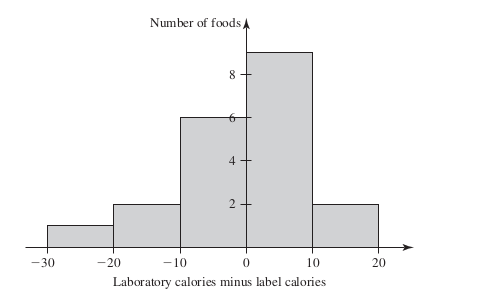
\includegraphics[width=0.5\textwidth]{img/7_3/img_2.png}

\end{figure}\vspace{1cm}

\subsection*{Amostragem de uma Distribuição Exponencial}

\noindent\textbf{Exemplo 7.3.11} \quad \textbf{Tempo de Vida de Componentes Eletrônicos.} No Exemplo 7.2.1, suponha que observemos os tempos de vida de três componentes, $X_1=3, X_2=1.5, X_3=2.1$. Eles foram modelados como i.i.d. variáveis exponenciais, dado $\theta$. Nossa distribuição a priori para $\theta$ foi a distribuição gama com parâmetros 1 e 2. Qual é a distribuição a posteriori de $\theta$ dados esses tempos de vida observados?

\vspace{1cm}
Ao amostrar de uma distribuição exponencial para a qual o valor do parâmetro $\theta$ é desconhecido, a família de distribuições gama serve como uma família conjugada de distribuições a priori, como mostrado no próximo teorema.

\vspace{1cm}
\noindent\textbf{Teorema 7.3.4} \quad Suponha que $X_1, \dots, X_n$ formem uma amostra aleatória de uma distribuição exponencial com parâmetro $\theta>0$ que é desconhecido. Suponha também que a distribuição a priori de $\theta$ seja a distribuição gama com parâmetros $\alpha>0$ e $\beta>0$. Então a distribuição a posteriori de $\theta$ dado que $X_i=x_i \, (i=1, \dots, n)$ é a distribuição gama com parâmetros $\alpha+n$ e $\beta+\sum_{i=1}^{n}x_i$.

\vspace{1cm}
\noindent\textbf{Prova} \quad Novamente, seja $y=\sum_{i=1}^{n}x_i$. Então a função de verossimilhança $f_n(\mathbf{x}|\theta)$ tem a forma
$$ f_n(\mathbf{x}|\theta) = \theta^n e^{-\theta y}. $$
Além disso, a f.d.p. a priori $\xi(\theta)$ tem a forma
$$ \xi(\theta) \propto \theta^{\alpha-1}e^{-\beta\theta} \quad \text{para } \theta>0. $$
Portanto, segue-se que a f.d.p. a posteriori $\xi(\theta|\mathbf{x})$ tem a forma
$$ \xi(\theta|\mathbf{x}) \propto \theta^{\alpha+n-1}e^{-(\beta+y)\theta} \quad \text{para } \theta>0. $$
O lado direito desta relação pode ser reconhecido como sendo, exceto por um fator constante, a f.d.p. da distribuição gama com parâmetros $\alpha+n$ e $\beta+y$. Portanto, a distribuição a posteriori de $\theta$ é como especificado no teorema. \rule{0.5em}{0.5em}

\vspace{1cm}
A distribuição a posteriori de $\theta$ no Teorema 7.3.4 depende do valor observado da estatística $Y = \sum_{i=1}^{n}X_i$; portanto, toda inferência sobre $\theta$ baseada na distribuição a posteriori dependerá do valor observado de $Y$.

\vspace{1cm}
\noindent\textbf{Exemplo 7.3.12} \quad \textbf{Tempo de Vida de Componentes Eletrônicos.} No Exemplo 7.3.11, podemos aplicar o Teorema 7.3.4 para encontrar a distribuição a posteriori. Na notação do teorema e sua prova, temos $n=3, \alpha=1, \beta=2$, e
$$ y = \sum_{i=1}^{n}x_i = 3+1.5+2.1=6.6. $$
A distribuição a posteriori de $\theta$ é então a distribuição gama com parâmetros $\alpha+n=1+3=4$ e $\beta+y=2+6.6=8.6$.
O leitor deve notar que o Teorema 7.3.4 teria encurtado muito a derivação da posterior no Exemplo 7.2.6.

\subsection*{Distribuições a Priori Impróprias}
Na Seção 7.2, mencionamos prioris impróprias como expedientes que tentam capturar a ideia de que há muito mais informação nos dados do que a contida em nossa distribuição a priori. Cada uma das famílias conjugadas que vimos nesta seção tem uma priori imprópria como um caso limite.

\vspace{1cm}
\noindent\textbf{Exemplo 7.3.13} \quad \textbf{Um Ensaio Clínico.} O que ilustramos aqui será aplicado a todos os exemplos em que os dados compreendem uma amostra i.i.d. (dado $\theta$) da distribuição de Bernoulli com parâmetro $\theta$. Considere os sujeitos no grupo da imipramina no Exemplo 2.1.4. A proporção de sucessos entre todos os pacientes que poderiam receber imipramina foi chamada de $P$ em exemplos anteriores, mas vamos chamá-la de $\theta$ desta vez para manter a notação geral deste capítulo. Suponha que $\theta$ tenha a distribuição beta com parâmetros $\alpha$ e $\beta$, e um conjugado geral a priori. Existem $n=40$ pacientes no grupo da imipramina, e 22 deles são sucessos. A distribuição a posteriori de $\theta$ é a distribuição beta com parâmetros $\alpha+22$ e $\beta+18$, como vimos no Teorema 7.3.1. A média da distribuição a posteriori é $(\alpha+22)/(\alpha+\beta+40)$. Se $\alpha$ e $\beta$ são pequenos, então a média a posteriori está próxima de 22/40, que é a proporção observada de sucessos. De fato, se $\beta=0$, o que não corresponde a uma distribuição beta real, então a média a posteriori é exatamente 22/40. No entanto, olhe o que acontece com $\alpha$ e $\beta$ quando eles se aproximam de 0. A f.d.p. beta (ignorando a constante) é $\theta^{\alpha-1}(1-\theta)^{\beta-1}$. Podemos definir $\alpha=\beta=0$ e fingir que $\xi(\theta) \propto \theta^{-1}(1-\theta)^{-1}$ é a f.d.p. a priori de $\theta$. A função de verossimilhança é $f_{40}(\mathbf{x}|\theta) = \binom{40}{22}\theta^{22}(1-\theta)^{18}$. Podemos ignorar o fator constante $\binom{40}{22}$ e obter o produto
$$ \xi(\theta|\mathbf{x}) \propto \theta^{21}(1-\theta)^{17}, \quad \text{para } 0<\theta<1. $$
Isso é facilmente reconhecido como sendo a mesma coisa que a f.d.p. da distribuição beta com parâmetros 22 e 18, exceto por um fator constante. Assim, se usarmos a "priori imprópria" beta com hiperparâmetros 0 e 0, obtemos a distribuição a posteriori beta para $\theta$ com hiperparâmetros 22 e 18. Note que o Teorema 7.3.1 produz a distribuição a posteriori correta mesmo neste caso de priori imprópria. A Figura 7.5 adiciona a f.d.p. da distribuição beta a posteriori calculada aqui à Fig. 2.4, que representava as probabilidades a posteriori para duas distribuições a priori discretas diferentes. Todas as três posteriores são muito próximas.

\vspace{1cm}
\begin{figure}[H]

\centering

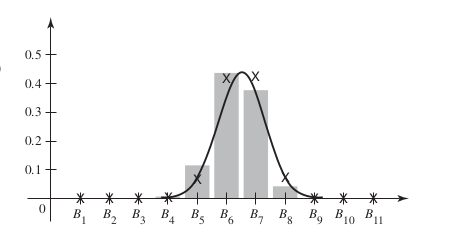
\includegraphics[width=0.5\textwidth]{img/7_3/img_3.png}

\end{figure}\vspace{1cm}

\noindent\textbf{Definição 7.3.2} \quad \textbf{Priori Imprópria.} Seja $\xi(\theta)$ uma função não negativa cujo domínio inclui o espaço de parâmetros de um modelo estatístico. Suponha que $\int \xi(\theta)d\theta = \infty$. Se pretendemos usar $\xi(\theta)$ como a f.d.p. a priori de $\theta$, então estamos usando uma \textit{priori imprópria} para $\theta$.

A Definição 7.3.2 não é muito útil para determinar uma priori imprópria a ser usada em uma aplicação particular. Existem muitos métodos para escolher uma priori imprópria, e a esperança é que todos eles levem a distribuições a posteriori semelhantes, de modo que não importe muito qual deles se escolhe. O método mais direto para escolher uma priori imprópria é começar com a família de distribuições conjugadas, se tal família existir. Na maioria dos casos, se a parametrização da família conjugada (hiperparâmetros) for escolhida com cuidado, a posteriori terá a mesma forma que a priori conjugada mais uma estatística. Alguém então substituiria cada um desses hiperparâmetros por 0 para obter o que parece ser a fórmula para a f.d.p. a posteriori. Isso é o que fizemos no Exemplo 7.3.13, cada um dos hiperparâmetros a posteriori era igual aos hiperparâmetros a priori correspondentes mais alguma estatística. Nesse exemplo, substituímos ambos os hiperparâmetros a priori por 0 para obter a priori imprópria. Aqui estão mais alguns exemplos.

No Teorema 7.3.2, os números $\alpha$ e $\beta$ são os hiperparâmetros a priori. Note que os hiperparâmetros a posteriori são $\alpha + \sum_{i=1}^{n}x_i$ e $\beta+n$. Note que a estatística $Y=\sum_{i=1}^{n}X_i$ é usada para calcular a distribuição a posteriori de $\theta$, e, portanto, fará parte de qualquer inferência baseada na posteriori.

\vspace{1cm}
\noindent\textbf{Exemplo 7.3.5} \quad \textbf{Chegadas de Clientes.} No Exemplo 7.3.4, podemos aplicar o Teorema 7.3.2 com $n=1, \alpha=3, \beta=2$, e $x_1=3$. A distribuição a posteriori de $\theta$ dado $X=3$ é a distribuição gama com parâmetros 6 e 3.

\vspace{1cm}
\noindent\textbf{Exemplo 7.3.6} \quad \textbf{A Variância da Distribuição Gama a Posteriori.} Considere uma distribuição de Poisson para a qual a média $\theta$ é desconhecida, e suponha que a f.d.p. a priori de $\theta$ seja a seguinte:
$$ \xi(\theta) = 
\begin{cases}
2e^{-2\theta} & \text{para } \theta>0, \\
0 & \text{para } \theta \le 0.
\end{cases}
$$
Suponha também que as observações devam ser retiradas da distribuição de Poisson até que a variância da distribuição a posteriori de $\theta$ tenha sido reduzida a 0.01 ou menos. Devemos determinar o número de observações que devem ser feitas antes que o processo de amostragem seja interrompido.
A f.d.p. a priori dada é a da distribuição gama com hiperparâmetros $\alpha=1$ e $\beta=2$. Portanto, depois de termos obtido valores observados $x_1, \dots, x_n$, a soma dos quais é $y=\sum_{i=1}^{n}x_i$, a distribuição a posteriori de $\theta$ será a distribuição gama com hiperparâmetros $y+1$ e $n+2$. Foi mostrado no Teorema 5.4.2 que a variância da distribuição gama com parâmetros $\alpha$ e $\beta$ é $\alpha/\beta^2$. Portanto, a variância $V$ da distribuição a posteriori de $\theta$ será
$$ V = \frac{y+1}{(n+2)^2}. $$
A amostragem deve parar assim que os valores observados $x_1, \dots, x_n$ forem tais que $V \le 0.01$. Ao contrário do Exemplo 7.3.2, não há limite uniforme sobre quão grande $n$ precisa ser porque $y$ pode ser arbitrariamente grande, não importa qual seja $n$. Claramente, são necessárias pelo menos $n=8$ observações antes que $V \le 0.01$.

\subsection*{Amostragem de uma Distribuição Normal}

\noindent\textbf{Exemplo 7.3.7} \quad \textbf{Emissões Automotivas.} Considere novamente o exemplo de emissões automotivas em Exemplo 5.6.1 na página 302. Antes de observar os dados, suponha que um engenheiro acreditasse que cada medida de emissão tinha a distribuição normal com média $\theta$ e desvio padrão 0.5, mas que $\theta$ era desconhecido. O engenheiro também acredita que $\theta$ tem uma distribuição normal com média 2.0 e desvio padrão 1.0. Depois de ver os dados na Fig. 5.1, como este engenheiro descreveria sua incerteza sobre $\theta$?

\vspace{1cm}
Quando as amostras são retiradas de uma distribuição normal para a qual o valor da média $\theta$ é desconhecido mas o valor da variância $\sigma^2$ é conhecido, a família de distribuições normais é uma família conjugada de distribuições a priori, como mostrado no próximo teorema.

\vspace{1cm}
\noindent\textbf{Teorema 7.3.3} \quad Suponha que $X_1, \dots, X_n$ formem uma amostra aleatória de uma distribuição normal para a qual o valor da média $\theta$ é desconhecido e o valor da variância $\sigma^2 > 0$ é conhecido. Suponha também que a distribuição a priori de $\theta$ seja uma distribuição normal com média $\mu_0$ e variância $\nu_0^2$. Então a distribuição a posteriori de $\theta$ dado que $X_i=x_i \, (i=1, \dots, n)$ é a distribuição normal com média $\mu_1$ e variância $\nu_1^2$, onde
\begin{equation}
\mu_1 = \frac{\sigma^2\mu_0+n\nu_0^2\bar{x}_n}{\sigma^2+n\nu_0^2} \tag{7.3.1}
\end{equation}
e
\begin{equation}
\nu_1^2 = \frac{\sigma^2\nu_0^2}{\sigma^2+n\nu_0^2}. \tag{7.3.2}
\end{equation}

\noindent\textbf{Prova} \quad A função de verossimilhança, $f_n(\mathbf{x}|\theta)$ tem a forma
$$ f_n(\mathbf{x}|\theta) \propto \exp\left[-\frac{1}{2\sigma^2}\sum_{i=1}^{n}(x_i-\theta)^2\right]. $$
Aqui, um fator constante foi descartado do lado direito. O método de completar o quadrado (ver Exercício 24 na Seção 5.6) nos diz que
$$ \sum_{i=1}^{n}(x_i-\theta)^2 = n(\theta-\bar{x}_n)^2 + \sum_{i=1}^{n}(x_i-\bar{x}_n)^2. $$
Omitindo um fator que envolve $x_1, \dots, x_n$ mas não depende de $\theta$, podemos reescrever $f_n(\mathbf{x}|\theta)$ na seguinte forma:
$$ f_n(\mathbf{x}|\theta) \propto \exp\left[-\frac{n}{2\sigma^2}(\theta-\bar{x}_n)^2\right]. $$
Como a f.d.p. a priori $\xi(\theta)$ tem a forma
$$ \xi(\theta) \propto \exp\left[-\frac{1}{2\nu_0^2}(\theta-\mu_0)^2\right], $$
segue-se que a f.d.p. a posteriori $\xi(\theta|\mathbf{x})$ satisfaz a relação
$$ \xi(\theta|\mathbf{x}) \propto \exp\left\{-\frac{1}{2}\left[\frac{n}{\sigma^2}(\theta-\bar{x}_n)^2+\frac{1}{\nu_0^2}(\theta-\mu_0)^2\right]\right\}. $$
Se $\mu_1$ e $\nu_1^2$ são como especificado nas Eqs. (7.3.1) e (7.3.2), completar o quadrado novamente estabelece a seguinte identidade:
$$ \frac{n}{\sigma^2}(\theta-\bar{x}_n)^2+\frac{1}{\nu_0^2}(\theta-\mu_0)^2 = \frac{1}{\nu_1^2}(\theta-\mu_1)^2 + \frac{n}{\sigma^2+n\nu_0^2}(\bar{x}_n-\mu_0)^2. $$
Como o termo final no lado direito desta equação não envolve $\theta$, ele pode ser absorvido na constante de proporcionalidade, e obtemos a relação
$$ \xi(\theta|\mathbf{x}) \propto \exp\left[-\frac{1}{2\nu_1^2}(\theta-\mu_1)^2\right]. $$
O lado direito desta relação pode ser reconhecido como sendo, exceto por um fator constante, a f.d.p. da distribuição normal com média $\mu_1$ e variância $\nu_1^2$. Portanto, a distribuição a posteriori de $\theta$ é como especificado no teorema. \rule{0.5em}{0.5em}

\vspace{1cm}
No Teorema 7.3.3, os números $\mu_0$ e $\nu_0^2$ são os hiperparâmetros a priori, enquanto $\mu_1$ e $\nu_1^2$ são os hiperparâmetros a posteriori. Note que a estatística $\bar{X}_n$ é usada na construção da distribuição a posteriori, e, portanto, desempenhará um papel em qualquer inferência baseada na posteriori.

\vspace{1cm}
\noindent\textbf{Exemplo 7.3.8} \quad \textbf{Emissões Automotivas.} Podemos aplicar o Teorema 7.3.3 para responder à pergunta no final do Exemplo 7.3.7. Na notação do teorema, temos $n=46, \sigma^2=0.5^2=0.25, \mu_0=2$ e $\nu_0^2=1.0$. A média das 46 medições é $\bar{x}_n=1.329$. A distribuição a posteriori de $\theta$ é então a distribuição normal com média e variância dadas por
$$ \mu_1 = \frac{0.25 \times 2 + 46 \times 1 \times 1.329}{0.25+46\times 1} = 1.333, $$
$$ \nu_1^2 = \frac{0.25 \times 1}{0.25+46\times 1} = 0.0054. $$
A média $\mu_1$ da distribuição a posteriori de $\theta$, como dada na Eq. (7.3.1), pode ser reescrita da seguinte forma:
\begin{equation}
\mu_1 = \frac{\sigma^2}{\sigma^2+n\nu_0^2}\mu_0 + \frac{n\nu_0^2}{\sigma^2+n\nu_0^2}\bar{x}_n. \tag{7.3.3}
\end{equation}
Pode-se ver da Eq. (7.3.3) que $\mu_1$ é uma média ponderada da média a priori $\mu_0$ e da média amostral $\bar{x}_n$. Além disso, pode-se ver que o peso relativo dado a $\bar{x}_n$ satisfaz as três propriedades a seguir: (1) Para valores fixos de $\nu_0^2$ e $\sigma^2$, quanto maior o tamanho da amostra $n$, maior será o peso relativo dado a $\bar{x}_n$. (2) Para valores fixos de $\nu_0^2$ e $n$, quanto maior a variância $\sigma^2$ de cada observação na amostra, menor será o peso relativo dado a $\bar{x}_n$. (3) Para valores fixos de $\sigma^2$ e $n$, quanto maior a variância $\nu_0^2$ da distribuição a priori, maior será o peso relativo dado a $\bar{x}_n$.
Além disso, pode-se ver da Eq. (7.3.2) que a variância $\nu_1^2$ da distribuição a posteriori de $\theta$ depende do número $n$ de observações que foram feitas, mas não depende das magnitudes dos valores observados. Portanto, para uma amostra aleatória de $n$ observações a ser retirada de uma distribuição normal para a qual o valor da média $\theta$ é desconhecido, o valor da variância é conhecido, e a distribuição a priori de $\theta$ é uma distribuição normal especificada. Então, antes de qualquer observação ter sido feita, podemos usar a Eq. (7.3.2) para calcular o valor da variância $\nu_1^2$ da distribuição a posteriori. No entanto, o valor da média $\mu_1$ da distribuição a posteriori dependerá dos valores observados que são obtidos na amostra. O fato de a variância a posteriori não depender dos valores observados deve-se à suposição de que a variância $\sigma^2$ das observações individuais é conhecida. Na Seção 8.6, relaxaremos essa suposição.

\vspace{1cm}
\noindent\textbf{Exemplo 7.3.9} \quad \textbf{A Variância da Distribuição Normal a Posteriori.} Suponha que as observações devam ser retiradas de uma distribuição normal com média $\theta$ e variância 1, e que o valor de $\theta$ seja desconhecido. Suponha também que a distribuição a priori de $\theta$ seja uma distribuição normal com variância 4. Além disso, as observações devem ser feitas até que a variância da distribuição a posteriori de $\theta$ tenha sido reduzida a 0.01 ou menos. Devemos determinar o número de observações que devem ser feitas antes que o processo de amostragem seja interrompido.
Segue-se da Eq. (7.3.2) que, após $n$ observações terem sido feitas, a variância $\nu_1^2$ da distribuição a posteriori será
$$ \nu_1^2 = \frac{4}{4n+1}. $$
Portanto, a relação $\nu_1^2 \le 0.01$ será satisfeita se e somente se $n \ge 99.75$. Portanto, a variância a posteriori será de 0.01 ou menos depois de 100 observações terem sido feitas e não antes.

\vspace{1cm}
\noindent\textbf{Exemplo 7.3.10} \quad \textbf{Contagem de Calorias em Alimentos Preparados.} Allison, Heshka, Sepulveda e Heymsfield (1993) amostraram 20 alimentos preparados nacionalmente e compararam o conteúdo de calorias declarado com o conteúdo de calorias determinado no laboratório. A Figura 7.4 é um histograma das diferenças percentuais entre as medições observadas em laboratório e o conteúdo de calorias anunciado nos rótulos dos alimentos. Suponha que modelamos a distribuição condicional das diferenças dado $\theta$ como a distribuição normal com média $\theta$ e variância 100. (Nesta seção, assumimos que a variância é conhecida. Na Seção 8.6, seremos capazes de lidar com o caso em que tanto a média quanto a variância são tratadas como variáveis aleatórias com uma distribuição conjunta.) Usaremos uma distribuição a priori para $\theta$ que é a distribuição normal com média 0 e uma variância de 60. Os dados $\mathbf{X}$ compreendem as 20 diferenças na Fig. 7.4, cuja média é 0.125. A distribuição a posteriori de $\theta$ seria então a distribuição normal com média
$$ \mu_1 = \frac{100 \times 0 + 20 \times 60 \times 0.125}{100+20\times 60} = 0.1154, $$
e variância
$$ \nu_1^2 = \frac{100 \times 60}{100+20\times 60} = 4.62. $$
Por exemplo, podemos estar interessados em saber se os empacotadores estão subestimando sistematicamente as calorias em seus alimentos em pelo menos 1 por cento. Isso corresponderia a $\theta > 1$. Usando o Teorema 5.6.6, podemos encontrar
$$ \Pr(\theta > 1|\mathbf{x}) = 1 - \Phi\left(\frac{1-0.1154}{\sqrt{4.62}}\right) = 1-\Phi(1.12) = 0.3403. $$
Há uma chance não desprezível, mas não esmagadora, de que os empacotadores estejam omitindo um por cento ou mais de suas calorias dos rótulos.

\vspace{1cm}
% [ESPAÇO PARA FIGURA 7.4]
\vspace{1cm}

\subsection*{Amostragem de uma Distribuição Exponencial}

\noindent\textbf{Exemplo 7.3.11} \quad \textbf{Tempo de Vida de Componentes Eletrônicos.} No Exemplo 7.2.1, suponha que observemos os tempos de vida de três componentes, $X_1=3, X_2=1.5, X_3=2.1$. Eles foram modelados como i.i.d. variáveis exponenciais, dado $\theta$. Nossa distribuição a priori para $\theta$ foi a distribuição gama com parâmetros 1 e 2. Qual é a distribuição a posteriori de $\theta$ dados esses tempos de vida observados?

\vspace{1cm}
Ao amostrar de uma distribuição exponencial para a qual o valor do parâmetro $\theta$ é desconhecido, a família de distribuições gama serve como uma família conjugada de distribuições a priori, como mostrado no próximo teorema.

\vspace{1cm}
\noindent\textbf{Teorema 7.3.4} \quad Suponha que $X_1, \dots, X_n$ formem uma amostra aleatória de uma distribuição exponencial com parâmetro $\theta>0$ que é desconhecido. Suponha também que a distribuição a priori de $\theta$ seja a distribuição gama com parâmetros $\alpha>0$ e $\beta>0$. Então a distribuição a posteriori de $\theta$ dado que $X_i=x_i \, (i=1, \dots, n)$ é a distribuição gama com parâmetros $\alpha+n$ e $\beta+\sum_{i=1}^{n}x_i$.

\vspace{1cm}
\noindent\textbf{Prova} \quad Novamente, seja $y=\sum_{i=1}^{n}x_i$. Então a função de verossimilhança $f_n(\mathbf{x}|\theta)$ tem a forma
$$ f_n(\mathbf{x}|\theta) = \theta^n e^{-\theta y}. $$
Além disso, a f.d.p. a priori $\xi(\theta)$ tem a forma
$$ \xi(\theta) \propto \theta^{\alpha-1}e^{-\beta\theta} \quad \text{para } \theta>0. $$
Portanto, segue-se que a f.d.p. a posteriori $\xi(\theta|\mathbf{x})$ tem a forma
$$ \xi(\theta|\mathbf{x}) \propto \theta^{\alpha+n-1}e^{-(\beta+y)\theta} \quad \text{para } \theta>0. $$
O lado direito desta relação pode ser reconhecido como sendo, exceto por um fator constante, a f.d.p. da distribuição gama com parâmetros $\alpha+n$ e $\beta+y$. Portanto, a distribuição a posteriori de $\theta$ é como especificado no teorema. \rule{0.5em}{0.5em}

\vspace{1cm}
A distribuição a posteriori de $\theta$ no Teorema 7.3.4 depende do valor observado da estatística $Y = \sum_{i=1}^{n}X_i$; portanto, toda inferência sobre $\theta$ baseada na distribuição a posteriori dependerá do valor observado de $Y$.

\vspace{1cm}
\noindent\textbf{Exemplo 7.3.12} \quad \textbf{Tempo de Vida de Componentes Eletrônicos.} No Exemplo 7.3.11, podemos aplicar o Teorema 7.3.4 para encontrar a distribuição a posteriori. Na notação do teorema e sua prova, temos $n=3, \alpha=1, \beta=2$, e
$$ y = \sum_{i=1}^{n}x_i = 3+1.5+2.1=6.6. $$
A distribuição a posteriori de $\theta$ é então a distribuição gama com parâmetros $\alpha+n=1+3=4$ e $\beta+y=2+6.6=8.6$.
O leitor deve notar que o Teorema 7.3.4 teria encurtado muito a derivação da posterior no Exemplo 7.2.6.

\subsection*{Distribuições a Priori Impróprias}
Na Seção 7.2, mencionamos prioris impróprias como expedientes que tentam capturar a ideia de que há muito mais informação nos dados do que a contida em nossa distribuição a priori. Cada uma das famílias conjugadas que vimos nesta seção tem uma priori imprópria como um caso limite.

\vspace{1cm}
\noindent\textbf{Exemplo 7.3.13} \quad \textbf{Um Ensaio Clínico.} O que ilustramos aqui será aplicado a todos os exemplos em que os dados compreendem uma amostra i.i.d. (dado $\theta$) da distribuição de Bernoulli com parâmetro $\theta$. Considere os sujeitos no grupo da imipramina no Exemplo 2.1.4. A proporção de sucessos entre todos os pacientes que poderiam receber imipramina foi chamada de $P$ em exemplos anteriores, mas vamos chamá-la de $\theta$ desta vez para manter a notação geral deste capítulo. Suponha que $\theta$ tenha a distribuição beta com parâmetros $\alpha$ e $\beta$, e um conjugado geral a priori. Existem $n=40$ pacientes no grupo da imipramina, e 22 deles são sucessos. A distribuição a posteriori de $\theta$ é a distribuição beta com parâmetros $\alpha+22$ e $\beta+18$, como vimos no Teorema 7.3.1. A média da distribuição a posteriori é $(\alpha+22)/(\alpha+\beta+40)$. Se $\alpha$ e $\beta$ são pequenos, então a média a posteriori está próxima de 22/40, que é a proporção observada de sucessos. De fato, se $\beta=0$, o que não corresponde a uma distribuição beta real, então a média a posteriori é exatamente 22/40. No entanto, olhe o que acontece com $\alpha$ e $\beta$ quando eles se aproximam de 0. A f.d.p. beta (ignorando a constante) é $\theta^{\alpha-1}(1-\theta)^{\beta-1}$. Podemos definir $\alpha=\beta=0$ e fingir que $\xi(\theta) \propto \theta^{-1}(1-\theta)^{-1}$ é a f.d.p. a priori de $\theta$. A função de verossimilhança é $f_{40}(\mathbf{x}|\theta) = \binom{40}{22}\theta^{22}(1-\theta)^{18}$. Podemos ignorar o fator constante $\binom{40}{22}$ e obter o produto
$$ \xi(\theta|\mathbf{x}) \propto \theta^{21}(1-\theta)^{17}, \quad \text{para } 0<\theta<1. $$
Isso é facilmente reconhecido como sendo a mesma coisa que a f.d.p. da distribuição beta com parâmetros 22 e 18, exceto por um fator constante. Assim, se usarmos a "priori imprópria" beta com hiperparâmetros 0 e 0, obtemos a distribuição a posteriori beta para $\theta$ com hiperparâmetros 22 e 18. Note que o Teorema 7.3.1 produz a distribuição a posteriori correta mesmo neste caso de priori imprópria. A Figura 7.5 adiciona a f.d.p. da distribuição beta a posteriori calculada aqui à Fig. 2.4, que representava as probabilidades a posteriori para duas distribuições a priori discretas diferentes. Todas as três posteriores são muito próximas.

\vspace{1cm}
% [ESPAÇO PARA FIGURA 7.5]
\vspace{1cm}

\noindent\textbf{Definição 7.3.2} \quad \textbf{Priori Imprópria.} Seja $\xi(\theta)$ uma função não negativa cujo domínio inclui o espaço de parâmetros de um modelo estatístico. Suponha que $\int \xi(\theta)d\theta = \infty$. Se pretendemos usar $\xi(\theta)$ como a f.d.p. a priori de $\theta$, então estamos usando uma \textit{priori imprópria} para $\theta$.

A Definição 7.3.2 não é muito útil para determinar uma priori imprópria a ser usada em uma aplicação particular. Existem muitos métodos para escolher uma priori imprópria, e a esperança é que todos eles levem a distribuições a posteriori semelhantes, de modo que não importe muito qual deles se escolhe. O método mais direto para escolher uma priori imprópria é começar com a família de distribuições conjugadas, se tal família existir. Na maioria dos casos, se a parametrização da família conjugada (hiperparâmetros) for escolhida com cuidado, a posteriori terá a mesma forma que a priori conjugada mais uma estatística. Alguém então substituiria cada um desses hiperparâmetros por 0 para obter o que parece ser a fórmula para a f.d.p. a posteriori. Isso é o que fizemos no Exemplo 7.3.13; cada um dos hiperparâmetros a posteriori era igual aos hiperparâmetros a priori correspondentes mais alguma estatística. Nesse exemplo, substituímos ambos os hiperparâmetros a priori por 0 para obter a priori imprópria. O método descrito anteriormente precisa ser modificado se alguém escolher uma parametrização "inconveniente" da priori conjugada, como no Exemplo 7.3.15 abaixo.

\vspace{1cm}
\noindent\textbf{Exemplo 7.3.14} \quad \textbf{Mortes no Exército Prussiano.} Bortkiewicz (1898) contou o número de soldados prussianos mortos por coices de cavalo em várias unidades do exército durante o século dezenove (um problema mais sério naquela época do que hoje). Havia 14 corpos do exército para cada um dos 20 anos, para um total de 280 contagens. As 280 contagens tiveram os seguintes valores: 144 contagens são 0, 91 contagens são 1, 32 contagens são 2, 11 contagens são 3, e 2 contagens são 4. Nenhuma unidade sofreu mais de quatro mortes por coices de cavalo em um único ano. (Esses dados foram reportados e analisados por Winsor, 1947.) Suponha que vamos modelar as 280 contagens como uma amostra aleatória de variáveis aleatórias de Poisson $X_1, \dots, X_{280}$ com média $\theta$ condicional ao parâmetro $\theta$. Uma priori conjugada seria um membro da família de distribuições gama com hiperparâmetros $\alpha$ e $\beta$. O Teorema 7.3.2 diz que a distribuição a posteriori de $\theta$ seria a distribuição gama com hiperparâmetros a posteriori 196 e 280, uma vez que a soma das 280 contagens é 196. A menos que $\alpha$ ou $\beta$ seja muito grande, a distribuição gama a posteriori é quase a mesma que a distribuição gama com hiperparâmetros posteriores 196 e 280. Este problema de distribuição a posteriori parece ser o resultado do uso de uma priori conjugada com hiperparâmetros a priori 0 e 0. Ignorando o fator constante, a f.d.p. da distribuição gama com parâmetros $\alpha$ e $\beta$ é $\theta^{\alpha-1}e^{-\beta\theta}$ para $\theta>0$. Se definirmos $\alpha=0$ e $\beta=0$ nesta fórmula, obtemos a "f.d.p. a priori imprópria" $\theta^{-1}$ para $\theta>0$. Fingindo que isso realmente era uma f.d.p. a priori e aplicando o teorema de Bayes para variáveis aleatórias (Teorema 3.6.4) resultaria em
$$ \xi(\theta|\mathbf{x}) \propto \theta^{195} e^{-280\theta}, \quad \text{para } \theta>0. $$
Isso é facilmente reconhecido como sendo a f.d.p. da distribuição gama com parâmetros 196 e 280, exceto por um fator constante. Este exemplo de resultado se aplica a todos os casos em que modelamos dados com distribuições de Poisson. A "distribuição gama" imprópria com hiperparâmetros a priori 0 e 0 pode ser usada no Teorema 7.3.2, e a conclusão ainda se manterá.

\vspace{1cm}
\noindent\textbf{Exemplo 7.3.15} \quad \textbf{Tempos de Falha de Rolamentos de Esferas.} Suponha que modelamos os 23 logaritmos de tempos de falha dos rolamentos de esferas do Exemplo 5.6.9 como variáveis aleatórias normais $X_1, \dots, X_{23}$ com média $\theta$ e variância 0.25. Uma priori conjugada para $\theta$ seria a distribuição normal com média $\mu_0$ e variância $\nu_0^2$. Para os log-tempos de falha, $\bar{x}_{23}=4.15$, então a distribuição a posteriori de $\theta$ seria a distribuição normal com média $\mu_1 = (0.25\mu_0+23 \times 4.15\nu_0^2)/(0.25+23\nu_0^2)$ e variância $\nu_1^2 = (0.25\nu_0^2)/(0.25+23\nu_0^2)$. Se deixarmos $\nu_0^2 \to \infty$ nas fórmulas para $\mu_1$ e $\nu_1^2$, obtemos $\mu_1 \to 4.15$ e $\nu_1^2 \to 0.25/23$. Ter variância infinita para a distribuição a priori de $\theta$ é como dizer que $\theta$ é igualmente provável de estar em qualquer lugar na reta real. Isso acontece em todos os exemplos em que modelamos dados $X_1, \dots, X_n$ como uma amostra aleatória da distribuição normal com média $\theta$ e variância conhecida $\sigma^2$ condicional a $\theta$. Se usarmos uma "distribuição normal" imprópria com variância infinita (a priori não precisa de média), o cálculo no Teorema 7.3.3 resultaria na distribuição normal com média $\bar{x}_n$ e variância $\sigma^2/n$. Neste caso, $\xi(\theta)$ seria igual a uma constante.
Este exemplo poderia ser uma aplicação do método descrito após a Definição 7.3.2 se tivéssemos os hiperparâmetros "mais convenientes": 1 sobre a variância $1/\nu_0^2$ e a média sobre a variância $\mu_0/\nu_0^2$. Em termos desses hiperparâmetros, a distribuição posterior tem 1 sobre sua variância igual a $1/\nu_1^2=1/\nu_0^2+n/\sigma^2=1/\nu_0^2+23/0.25$ e média sobre variância igual a $\mu_1/\nu_1^2 = \mu_0/\nu_0^2+23 \times 4.15/0.25$. Cada um dos hiperparâmetros a posteriori tem a forma do hiperparâmetro a priori correspondente mais uma estatística. A priori imprópria com a média sobre variância e 1 sobre variância iguais a 0 também tem $\xi(\theta)$ igual a uma constante.

\vspace{1cm}
Existem outros exemplos de prioris impróprias para outros modelos de amostragem. O leitor pode verificar (no Exercício 21) que a "distribuição gama" com parâmetros 0 e 0 leva a resultados semelhantes aos de uma amostra aleatória de uma distribuição exponencial. Os Exercícios 23 e 24 introduzem uma coleção geral de f.d.p.s $f(x|\theta)$ para as quais é fácil construir prioris impróprias.
Prioris impróprias foram introduzidas para casos em que os dados observados continham muito mais informação do que nossa distribuição a priori. Implicitamente, estamos assumindo que os dados são informativos. Quando os dados não contêm muita informação, as prioris impróprias podem ser altamente inapropriadas.

\vspace{1cm}
\noindent\textbf{Exemplo 7.3.16} \quad \textbf{Eventos Muito Raros.} No Exemplo 5.4.7, estávamos discutindo um contaminante de água potável conhecido como criptosporídio que geralmente ocorre em concentrações muito baixas. Suponha que uma autoridade de água modele os oocistos de criptosporídio no abastecimento de água como um processo de Poisson com taxa de $\theta$ oocistos por litro. Eles decidem amostrar 25 litros de água para aprender sobre $\theta$. Suponha que eles usem a priori gama imprópria com "f.d.p." $\theta^{-1}$. (Esta é a mesma priori imprópria usada no Exemplo 7.3.14.) Se a amostra de 25 litros não contiver oocistos, a autoridade de água teria uma distribuição a posteriori para $\theta$ que é a distribuição gama com parâmetros 0 e 5, o que não é uma distribuição real. Não importa quantos litros eles amostrem, a distribuição a posteriori não será uma distribuição real até que pelo menos um oocisto seja observado. Ao amostrar eventos raros, pode-se ser forçado a quantificar a informação a priori na forma de uma distribuição a priori adequada para fazer inferências baseadas na distribuição a posteriori.

\subsection*{Resumo}
Para cada uma das várias famílias diferentes de modelos estatísticos, para dados de uma determinada família, encontramos uma família conjugada de distribuições para o parâmetro. Essas famílias têm a propriedade de que, se a distribuição a priori for escolhida da família, então a distribuição a posteriori é um membro da família. Para dados com distribuições relacionadas à Bernoulli, como binomial, geométrica e binomial negativa, a família conjugada para o parâmetro de sucesso é a família de distribuições beta. Para dados com distribuições relacionadas ao processo de Poisson, como Poisson e gama (com primeiro parâmetro conhecido), e exponencial, a família conjugada para o parâmetro de taxa é a família de distribuições gama. Para dados com uma distribuição normal com variância conhecida, a família conjugada para a média é a família normal. Também descrevemos o uso de prioris impróprias. Prioris impróprias não são distribuições de probabilidade, mas se fingirmos que são, podemos calcular distribuições a posteriori que se aproximam daquelas que teríamos obtido usando prioris conjugadas apropriadas com valores extremos dos hiperparâmetros a priori.

\section*{Exercícios}
\begin{enumerate}
    \item Considere novamente a situação descrita no Exemplo 7.3.10. Uma vez mais, suponha que a distribuição a priori de $\theta$ seja uma distribuição normal com média 0, mas desta vez seja a variância a priori $\nu_0^2 > 0$. Se a média a posteriori de $\theta$ for 0.12, que valor de $\nu_0^2$ foi usado?
    
    \item Mostre que no Exemplo 7.3.2 deve-se ter $V \le 0.01$ depois que 22 itens tiverem sido selecionados. Mostre também que $V > 0.01$ até que pelo menos sete itens tenham sido selecionados.
    
    \item Suponha que a proporção $\theta$ de itens defeituosos em um grande lote seja desconhecida e que a distribuição a priori de $\theta$ seja a distribuição beta com parâmetros 2 e 200. Se 100 itens forem selecionados aleatoriamente do lote e três deles forem defeituosos, qual é a distribuição a posteriori de $\theta$?
    
    \item Considere novamente as condições do Exercício 3. Suponha que, depois de observar três itens defeituosos entre os 100 itens selecionados, a distribuição a posteriori de $\theta$ que um estatístico atribui seja uma distribuição beta para a qual a média é 2/51 e a variância é $98/(51^2(103))$. Que distribuição a priori o estatístico atribuiu a $\theta$?
    
    \item Suponha que o número de defeitos em um rolo de 1200 pés de fita magnética tenha uma distribuição de Poisson para a qual o valor da média $\theta$ é desconhecido, e a distribuição a priori de $\theta$ seja a distribuição gama com parâmetros $\alpha=3$ e $\beta=1$. Quando cinco rolos desta fita são selecionados e inspecionados, o número de defeitos encontrados neles são 2, 2, 6, 0 e 3. Determine a distribuição a posteriori de $\theta$.
    
    \item Seja $\theta$ o número médio de defeitos por 100 pés de um certo tipo de fita magnética. Suponha que o valor de $\theta$ seja desconhecido e que a distribuição a priori de $\theta$ seja a distribuição gama com parâmetros $\alpha=2$ e $\beta=10$. Quando um rolo de 1200 pés desta fita é inspecionado, exatamente quatro defeitos são encontrados. Determine a distribuição a posteriori de $\theta$.
    
    \item Suponha que as alturas dos indivíduos em uma certa população tenham uma distribuição normal para a qual o valor da média $\theta$ é desconhecido e o desvio padrão é 2 polegadas. Suponha também que a distribuição a priori de $\theta$ seja uma distribuição normal para a qual a média é 68 polegadas e o desvio padrão é 1 polegada. Se 10 pessoas forem selecionadas aleatoriamente da população, e sua altura média for de 69.5 polegadas, qual é a distribuição a posteriori de $\theta$?
    
    \item Considere novamente o problema descrito no Exercício 7.
    \begin{enumerate}[label=(\alph*)]
        \item Qual intervalo de 1 polegada de comprimento tem a maior probabilidade a priori de conter o valor de $\theta$?
        \item Qual intervalo de 1 polegada de comprimento tem a maior probabilidade a posteriori de conter o valor de $\theta$?
        \item Encontre as probabilidades dos intervalos nas partes (a) e (b).
    \end{enumerate}
    
    \item Suponha que uma amostra aleatória de 20 observações seja retirada de uma distribuição normal para a qual o valor da média $\theta$ é desconhecido e a variância é 1. Depois que os valores tiverem sido observados, descobre-se que $\bar{x}_n=10$, e que a distribuição a posteriori de $\theta$ é uma distribuição normal para a qual a média é 8 e a variância é 1/25. Qual foi a distribuição a priori de $\theta$?
    
    \item Suponha que uma amostra aleatória de 2 observações deva ser retirada de uma distribuição normal para a qual o valor da média $\theta$ é desconhecido e o desvio padrão é 2, e a distribuição a priori de $\theta$ seja uma distribuição normal com o desvio padrão 1. Qual é o menor número de observações que devem ser incluídas na amostra para reduzir o desvio padrão da distribuição a posteriori de $\theta$ para o valor 0.1?
    
    \item Suponha que uma amostra aleatória de 100 observações seja retirada de uma distribuição normal para a qual o valor da média $\theta$ é desconhecido e o desvio padrão é $\sigma$. Suponha que a distribuição a priori de $\theta$ seja uma distribuição normal. Mostre que, não importa qual seja o desvio padrão da distribuição a priori, o desvio padrão da distribuição a posteriori será menor que $\sigma/5$.
    
    \item Suponha que o tempo em minutos necessário para servir um cliente em um caixa de banco tenha uma distribuição exponencial para a qual o valor do parâmetro $\beta$ é desconhecido, e a distribuição a priori de $\beta$ seja uma distribuição gama para a qual a média é 0.2 e o desvio padrão é 1. Se o tempo médio necessário para servir uma amostra aleatória de 20 clientes for de 3.5 minutos, qual é a distribuição a posteriori de $\beta$?
    
    \item Para uma distribuição com média $\mu \ne 0$ e desvio padrão $\sigma>0$, o \textit{coeficiente de variação} da distribuição é definido como $\sigma/|\mu|$. Considere novamente o problema descrito no Exercício 12, e suponha que o coeficiente de variação da distribuição gama a priori de $\beta$ seja 2. Qual é o menor número de clientes que devem ser observados para reduzir o coeficiente de variação da distribuição a posteriori para 0.1?
    
    \item Mostre que a família de distribuições beta é uma família conjugada de distribuições a priori para amostras de uma distribuição binomial negativa com um valor conhecido do parâmetro $r$ e um valor desconhecido do parâmetro $p \, (0<p<1)$.
    
    \item Seja $\xi(\theta)$ uma f.d.p. definida da seguinte forma para constantes $\alpha > 0$ e $\beta > 0$:
    $$ \xi(\theta) = 
    \begin{cases}
        \frac{\beta^\alpha}{\Gamma(\alpha)}\theta^{-(\alpha+1)}e^{-\beta/\theta} & \text{para } \theta>0, \\
        0 & \text{para } \theta \le 0.
    \end{cases}
    $$
    Uma distribuição com esta f.d.p. é chamada de \textit{distribuição gama inversa}.
    \begin{enumerate}[label=(\alph*)]
        \item Verifique se $\xi(\theta)$ é realmente uma f.d.p. verificando que $\int_0^\infty \xi(\theta)d\theta = 1$.
        \item Considere a família de distribuições de probabilidade que pode ser representada por uma f.d.p. $\xi(\theta)$ tendo a forma geral dada para todos os pares de constantes $\alpha>0$ e $\beta>0$ possíveis. Mostre que esta família é uma família conjugada de distribuições a priori para amostras de uma distribuição normal com um valor conhecido da média $\mu$ e um valor desconhecido da variância $\theta$.
    \end{enumerate}
    
    \item No Exercício 15, o parâmetro é considerado o desvio padrão em vez da variância. Determine uma família conjugada de distribuições a priori para amostras de uma distribuição normal com um valor conhecido da média $\mu$ e um valor desconhecido do desvio padrão $\sigma$.
    
    \item Suponha que o número de minutos que uma pessoa deve esperar por um ônibus a cada manhã tenha a distribuição uniforme no intervalo $[0, \theta]$, onde o valor do ponto final $\theta$ é desconhecido. Suponha também que a f.d.p. a priori de $\theta$ seja a seguinte:
    $$ \xi(\theta) = 
    \begin{cases}
        \frac{192}{\theta^4} & \text{para } \theta \ge 4, \\
        0 & \text{caso contrário.}
    \end{cases}
    $$
    Se os tempos de espera observados em três manhãs sucessivas forem 5, 3 e 8 minutos, qual é a f.d.p. a posteriori de $\theta$?
    
    \item A distribuição de Pareto com parâmetros $x_0$ e $\alpha \, (x_0>0$ e $\alpha>0)$ é definida no Exercício 16 da Seção 5.7. Mostre que a família de distribuições de Pareto é uma família conjugada de distribuições a priori para amostras de uma distribuição uniforme no intervalo $[0, \theta]$, onde o valor do ponto final $\theta$ é desconhecido.
    
    \item Suponha que $X_1, \dots, X_n$ formem uma amostra aleatória de uma distribuição para a qual a f.d.p. $f(x|\theta)$ é a seguinte:
    $$ f(x|\theta) = 
    \begin{cases}
        \theta x^{\theta-1} & \text{para } 0 < x < 1, \\
        0 & \text{caso contrário.}
    \end{cases}
    $$
    Suponha também que o valor do parâmetro $\theta$ seja desconhecido $(\theta>0)$, e a distribuição a priori de $\theta$ seja uma distribuição gama com parâmetros $\alpha$ e $\beta \, (\alpha>0$ e $\beta>0)$. Determine a média e a variância da distribuição a posteriori de $\theta$.
    
    \item Suponha que modelamos os tempos de vida (em meses) de componentes eletrônicos como variáveis aleatórias exponenciais independentes com parâmetro desconhecido $\beta$. Modelamos $\beta$ como tendo uma distribuição gama com parâmetros $a$ e $b$. Acreditamos que o tempo de vida médio é de quatro meses, com um desvio padrão de seis meses. Também observamos 10 componentes com uma vida útil média observada de cinco meses. Determine a média e o desvio padrão da vida útil média, dado que observamos os 10 componentes. Dica: use o Exercício 21 da Seção 5.7.
    
    \item Suponha que $X_1, \dots, X_n$ formem uma amostra aleatória de uma distribuição exponencial com parâmetro $\theta$. Seja a priori para $\theta$ imprópria com "f.d.p." $\xi(\theta) = 1/\theta$ para $\theta>0$. Encontre a distribuição a posteriori de $\theta$ e mostre que a média a posteriori de $\theta$ é $1/\bar{x}_n$.
    
    \item Considere os dados no Exemplo 7.3.10. Desta vez, suponha que usemos a priori imprópria "f.d.p." $\xi(\theta) = 1$ para todo $\theta$. Encontre a distribuição a posteriori de $\theta$ e a probabilidade a posteriori de que $\theta>1$.
    
    \item Considere uma distribuição para a qual a f.d.p. ou f.p. $f(x|\theta)$ é tal que $\theta$ pertence a algum espaço de parâmetros $\Omega$. É dito que uma família de distribuições obtidas deixando $\theta$ variar em $\Omega$ é uma \textit{família exponencial}, ou uma \textit{família de Koopman-Darmois}, se $f(x|\theta)$ pode ser escrito da seguinte forma para $\theta \in \Omega$ e todos os valores de $x$:
    $$ f(x|\theta) = a(\theta)b(x)\exp[c(\theta)d(x)]. $$
    Aqui $a(\theta)$ e $c(\theta)$ são funções arbitrárias de $\theta$, e $b(x)$ e $d(x)$ são funções arbitrárias de $x$.
    Para cada um $(a, \beta) \in H$, seja
    $$ \xi_{a, \beta}(\theta) = \frac{[a(\theta)]^\beta \exp[\alpha c(\theta)]}{\int_H [a(\eta)]^\beta \exp[\alpha c(\eta)] d\eta}. $$
    Seja $\Psi$ o conjunto de todas as distribuições de probabilidade que têm f.d.p.s da forma $\xi_{a, \beta}(\theta)$ para alguns $(a, \beta) \in H$.
    \begin{enumerate}[label=(\alph*)]
        \item Mostre que $\Psi$ é uma família conjugada de distribuições a priori para amostras de $\Psi$.
        \item Suponha que observamos uma amostra aleatória de tamanho $n$ da distribuição com f.d.p. $f(x|\theta)$. Se a f.d.p. a priori de $\theta$ for $\xi_{\alpha_0, \beta_0}$, mostre que os hiperparâmetros a posteriori são
        $$ \alpha_1 = \alpha_0+n, \beta_1 = \beta_0 + \sum_{i=1}^{n}d(x_i). $$
    \end{enumerate}
    
    \item Mostre que cada uma das seguintes famílias de distribuições é uma família exponencial, como definido no Exercício 23.
    \begin{enumerate}[label=(\alph*)]
        \item A família de distribuições de Bernoulli com um valor desconhecido do parâmetro $p$.
        \item A família de distribuições de Poisson com uma média desconhecida.
        \item A família de distribuições binomiais negativas para as quais o valor de $r$ é conhecido e o valor de $p$ é desconhecido.
        \item A família de distribuições normais com uma média desconhecida e uma variância conhecida.
        \item A família de distribuições normais com uma variância desconhecida e uma média conhecida.
        \item A família de distribuições gama para as quais o valor de $\alpha$ é conhecido e o valor de $\beta$ é desconhecido.
        \item A família de distribuições gama para as quais o valor de $\beta$ é conhecido e o valor de $\alpha$ é desconhecido.
        \item A família de distribuições beta para as quais o valor de $\alpha$ é conhecido e o valor de $\beta$ é desconhecido.
    \end{enumerate}

    \item Mostre que a família de distribuições uniformes nos intervalos $[0, \theta]$ para $\theta>0$ não é uma família exponencial, como definido no Exercício 23. Olhe para o suporte de cada distribuição.
    
    \item Mostre que a família de distribuições uniformes discretas nos conjuntos $\{0, 1, \dots, \theta\}$ para um inteiro não negativo $\theta$ não é uma família exponencial, como definido no Exercício 23.

\end{enumerate}